\fancychapter{Results: Pirate Game}
\label{ap:d}

\section{$3$ Player Game}

\subsection{ Captain proposes $(99,0,1)$.}
 
\subsubsection{ Accepted proposal after 1 round of the game.}

\begin{table}[ht]
\begin{center}

\begin{tabular}{cc}
  a)\putindeepbox[7pt]{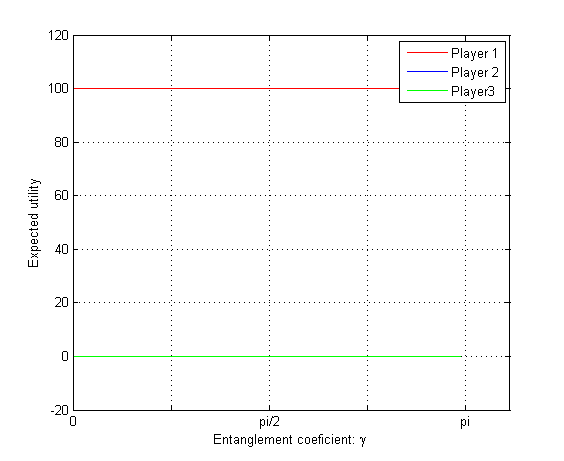
\includegraphics[scale=0.46]{3Accepted99/CCC.PNG}}
    & a1)\putindeepbox[7pt]{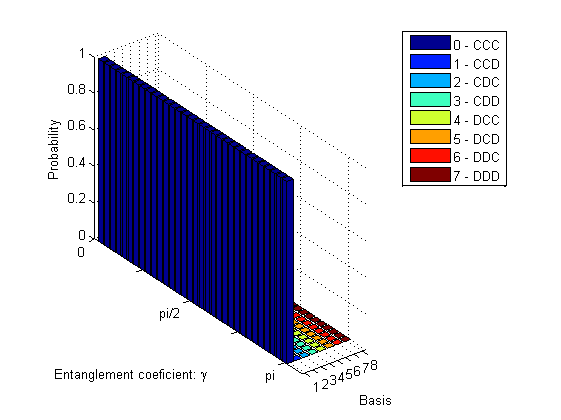
\includegraphics[scale=0.46]{3Accepted99/CCC_1.PNG}} \\
\end{tabular}
\caption{a) Expected utility for $3$ players, where the players will use the $(Cooperate, Cooperate, Cooperate)$ operators. The initial proposal is $(\alpha_{1}, \alpha_{2}, \alpha_{3}) =(99, 0, 1)$. a1) Probability distribution of the final state depending on the entanglement coefficient $\gamma$. }
\label{tab:3playerCCC99}
\end{center}
 \end{table}

\begin{table}[h]
\begin{center}
\begin{tabular}{cc}
  b)\putindeepbox[7pt]{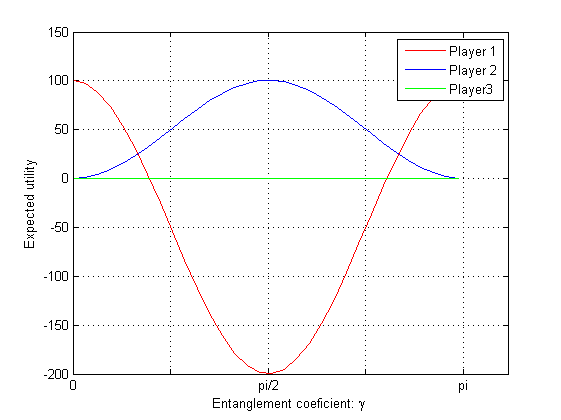
\includegraphics[scale=0.46]{3Accepted99/CCD.PNG}}
    & b1)\putindeepbox[7pt]{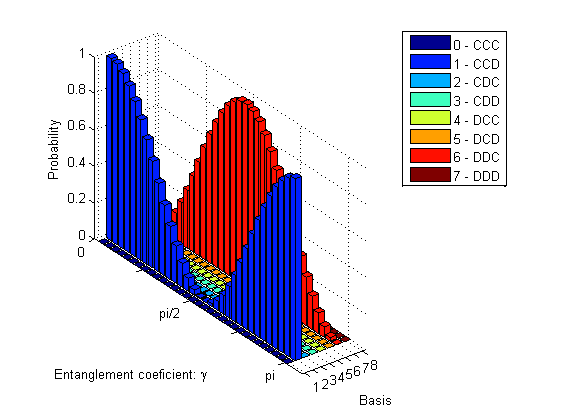
\includegraphics[scale=0.46]{3Accepted99/CCD_1.PNG}} \\
\end{tabular}
\caption{b) Expected utility for $3$ players, where the players will use the $(Cooperate, Cooperate, Defect)$ operators. b1) Probability distribution of the final state depending on the entanglement coefficient $\gamma$. }
\label{tab:3playerCCD99}
\end{center}
 \end{table}

\begin{table}[h]
\begin{center}
\begin{tabular}{cc}
  c)\putindeepbox[7pt]{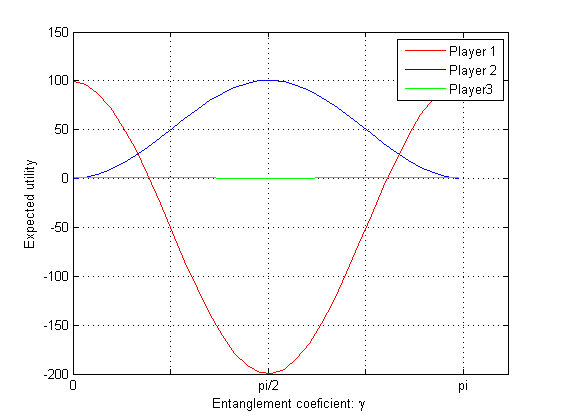
\includegraphics[scale=0.46]{3Accepted99/CDC.PNG}}
    & c1)\putindeepbox[7pt]{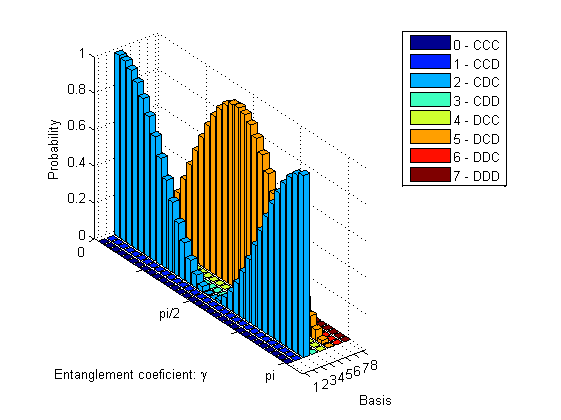
\includegraphics[scale=0.46]{3Accepted99/CDC_1.PNG}} \\
\end{tabular}
\caption{c) Expected utility for $3$ players, where the players will use the $(Cooperate, Defect, Cooperate)$ operators. c1) Probability distribution of the final state depending on the entanglement coefficient $\gamma$. }
\label{tab:3playerCDC99}
\end{center}
 \end{table}

\begin{table}[h]
\begin{center}
\begin{tabular}{cc}
  d)\putindeepbox[7pt]{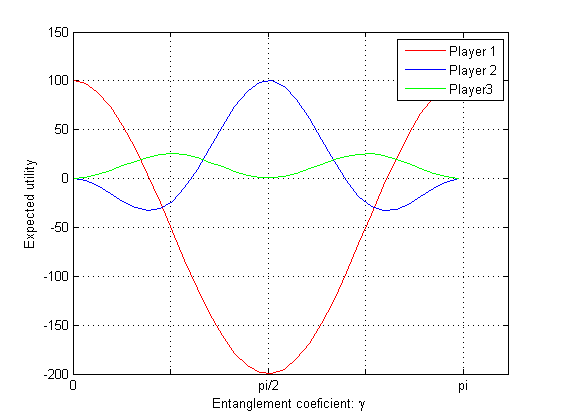
\includegraphics[scale=0.46]{3Accepted99/DCC.PNG}}
    & d1)\putindeepbox[7pt]{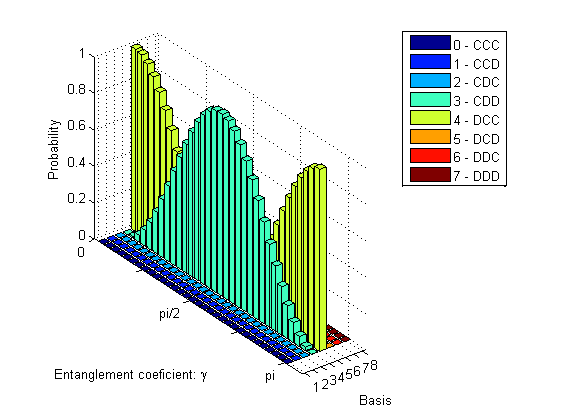
\includegraphics[scale=0.46]{3Accepted99/DCC_1.PNG}} \\
\end{tabular}
\caption{b) Expected utility for $3$ players, where the players will use the $(Defect, Cooperate, Cooperate)$ operators. b1) Probability distribution of the final state depending on the entanglement coefficient $\gamma$. }
\label{tab:3playerDCC99}
\end{center}
 \end{table}

\clearpage
\subsubsection{Initial proposal rejected; $(Cooperate , Defect, Defect)$}

%\item  Rejected proposal after 1 round of the game.\\

%\begin{itemize}

%\item In the first round the players use the operators $(CDD)$.\\

\begin{table}[h]
\begin{center}
\begin{tabular}{cc}
  a)\putindeepbox[7pt]{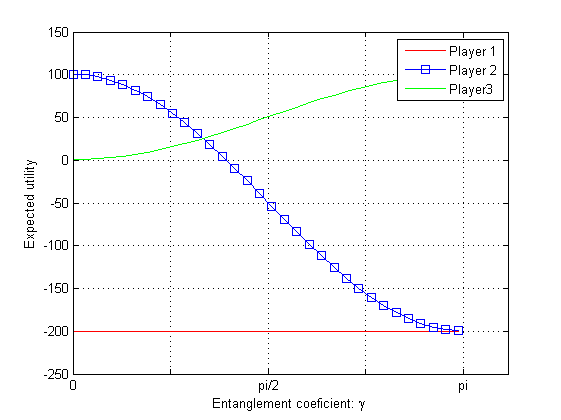
\includegraphics[scale=0.46]{3Rejected99/CDD_CC.PNG}}
    & a1)\putindeepbox[7pt]{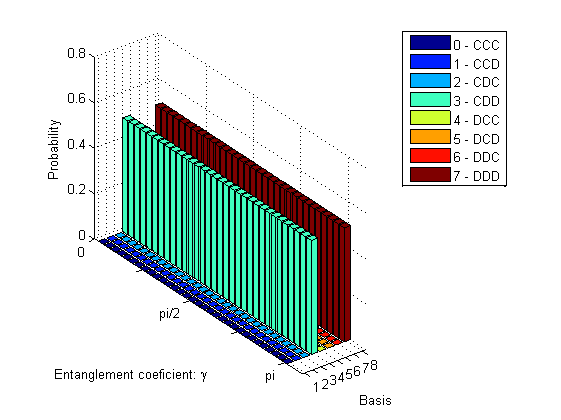
\includegraphics[scale=0.46]{3Rejected99/CDD_CC1.PNG}} \\
\end{tabular}
\caption{a) Expected utility for $3$ players, where the players will use the $(Cooperate , Defect, Defect)$ operators in the first round of the game; in the second round player 2 and player 3 will play $(CC)$. }
\label{tab:3playerCDD_CC99}
\end{center}
 \end{table}

\begin{table}[h]
\begin{center}
\begin{tabular}{cc}
  b)\putindeepbox[7pt]{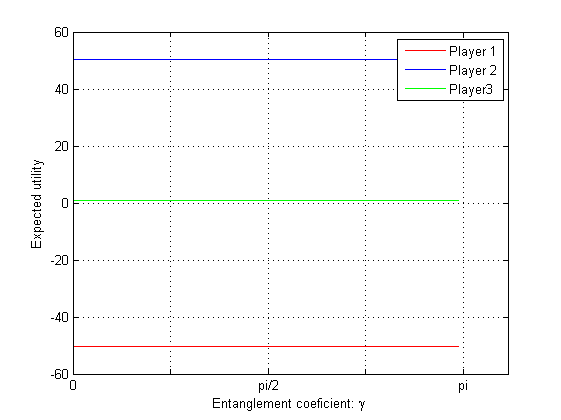
\includegraphics[scale=0.46]{3Rejected99/CDD_CD.PNG}}
    & b1)\putindeepbox[7pt]{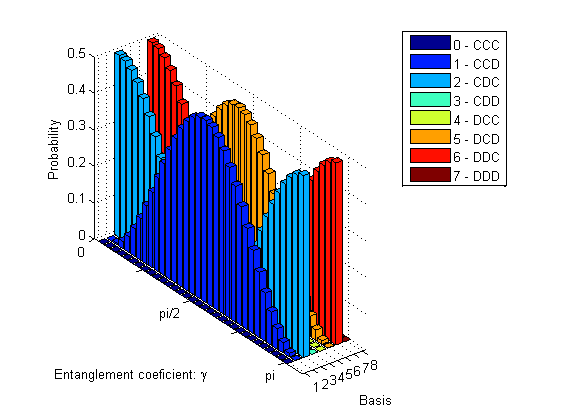
\includegraphics[scale=0.46]{3Rejected99/CDD_CD1.PNG}} \\
\end{tabular}
\caption{b) Expected utility for $3$ players, where the players will use the $(Cooperate , Defect, Defect)$ operators in the first round of the game; in the second round player 2 and player 3 will play $(CD)$. }
\label{tab:3playerCDD_CD99}
\end{center}
 \end{table}

\begin{table}[h]
\begin{center}
\begin{tabular}{cc}
  c)\putindeepbox[7pt]{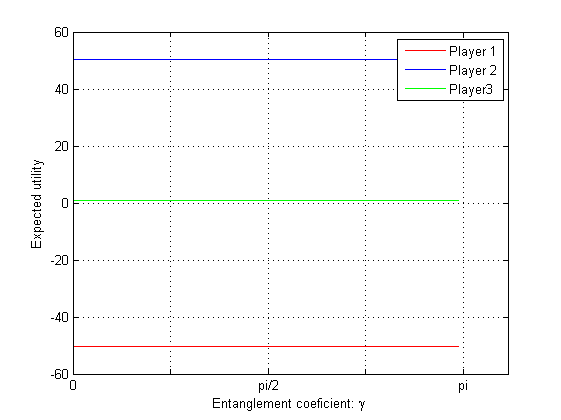
\includegraphics[scale=0.46]{3Rejected99/CDD_DC.PNG}}
    & c1)\putindeepbox[7pt]{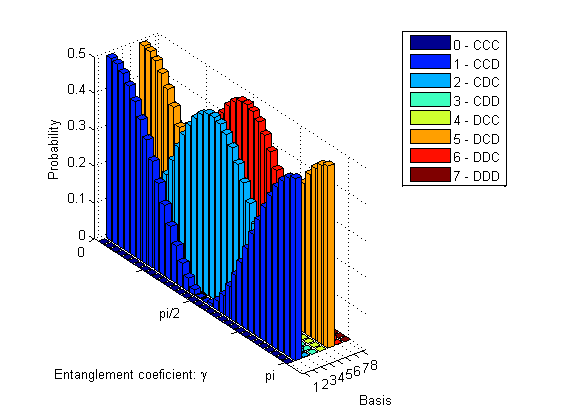
\includegraphics[scale=0.46]{3Rejected99/CDD_DC1.PNG}} \\
\end{tabular}
\caption{c) Expected utility for $3$ players, where the players will use the $(Cooperate , Defect, Defect)$ operators in the first round of the game; in the second round player 2 and player 3 will play $(DC)$. }
\label{tab:3playerCDD_DC99}
\end{center}
 \end{table}

\begin{table}[h]
\begin{center}
\begin{tabular}{cc}
  d)\putindeepbox[7pt]{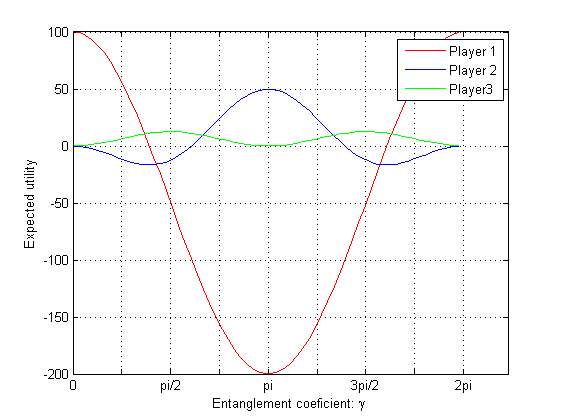
\includegraphics[scale=0.46]{3Rejected99/CDD_DD.PNG}}
    & d1)\putindeepbox[7pt]{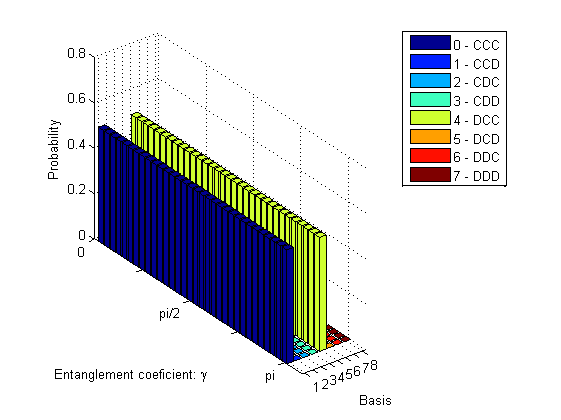
\includegraphics[scale=0.46]{3Rejected99/CDD_DD1.PNG}} \\
\end{tabular}
\caption{b) Expected utility for $3$ players, where the players will use the $(Cooperate , Defect, Defect)$ operators in the first round of the game; in the second round player 2 and player 3 will play $(DD)$. }
\label{tab:3playerCDD_DD99}
\end{center}
 \end{table}


\clearpage
\subsubsection{Initial proposal rejected; $(Defect, Cooperate, Defect)$}

\begin{table}[h]
\begin{center}
\begin{tabular}{cc}
  a)\putindeepbox[7pt]{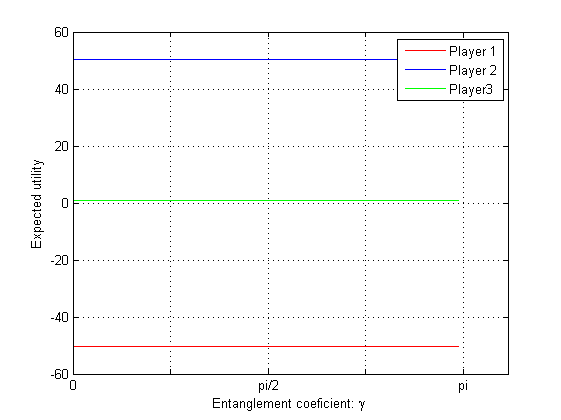
\includegraphics[scale=0.46]{3Rejected99/DCD_CC.PNG}}
    & a1)\putindeepbox[7pt]{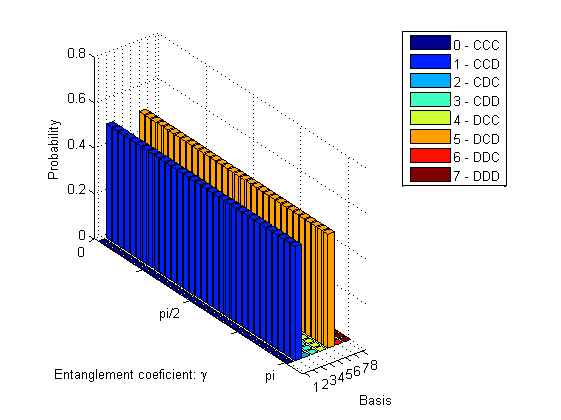
\includegraphics[scale=0.46]{3Rejected99/DCD_CC1.PNG}} \\
\end{tabular}
\caption{a) Expected utility for $3$ players, where the players will use the $(Defect, Cooperate, Defect)$ operators in the first round of the game; in the second round player 2 and player 3 will play $(CC)$. }
\label{tab:3playerDCD_CC99}
\end{center}
 \end{table}

\begin{table}[h]
\begin{center}
\begin{tabular}{cc}
  b)\putindeepbox[7pt]{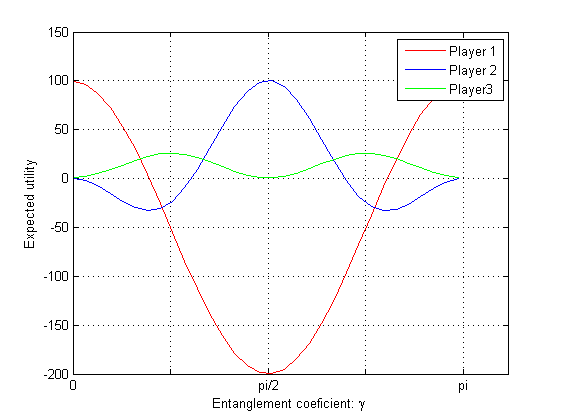
\includegraphics[scale=0.46]{3Rejected99/DCD_CD.PNG}}
    & b1)\putindeepbox[7pt]{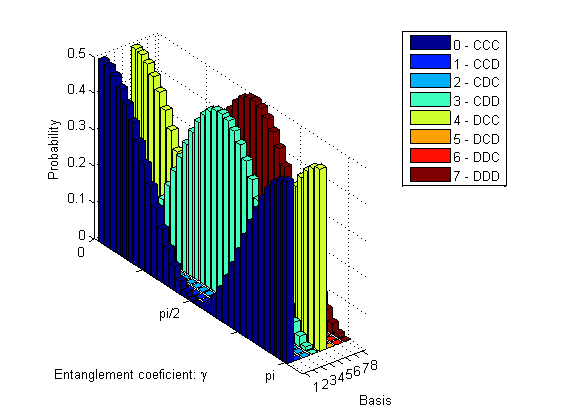
\includegraphics[scale=0.46]{3Rejected99/DCD_CD1.PNG}} \\
\end{tabular}
\caption{b) Expected utility for $3$ players, where the players will use the $(Defect, Cooperate, Defect)$ operators in the first round of the game; in the second round player 2 and player 3 will play $(CD)$. }
\label{tab:3playerDCD_CD99}
\end{center}
 \end{table}

\begin{table}[h]
\begin{center}
\begin{tabular}{cc}
  c)\putindeepbox[7pt]{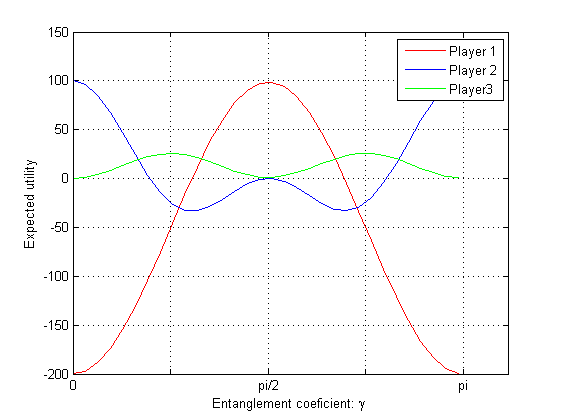
\includegraphics[scale=0.46]{3Rejected99/DCD_DC.PNG}}
    & c1)\putindeepbox[7pt]{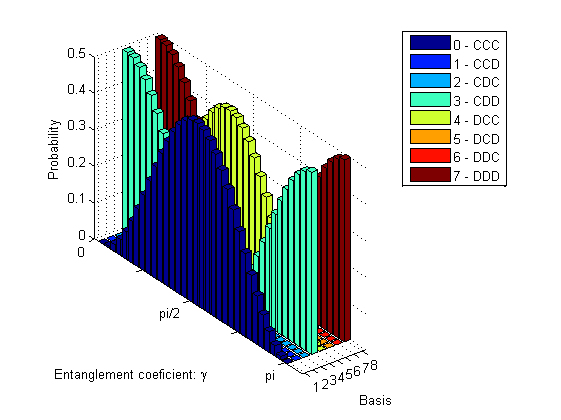
\includegraphics[scale=0.46]{3Rejected99/DCD_DC1.PNG}} \\
\end{tabular}
\caption{c) Expected utility for $3$ players, where the players will use the $(Defect, Cooperate, Defect)$ operators in the first round of the game; in the second round player 2 and player 3 will play $(DC)$. }
\label{tab:3playerDCD_DC99}
\end{center}
 \end{table}

\begin{table}[h]
\begin{center}
\begin{tabular}{cc}
  d)\putindeepbox[7pt]{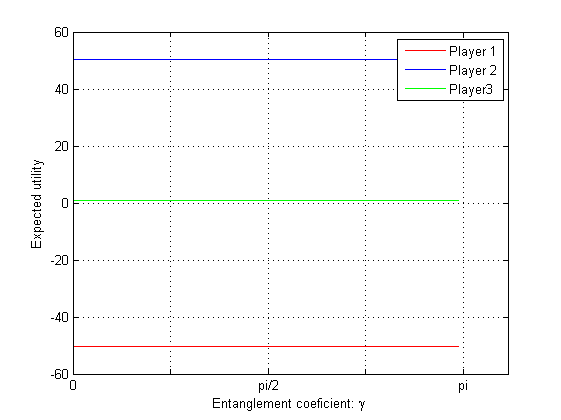
\includegraphics[scale=0.46]{3Rejected99/DCD_DD.PNG}}
    & d1)\putindeepbox[7pt]{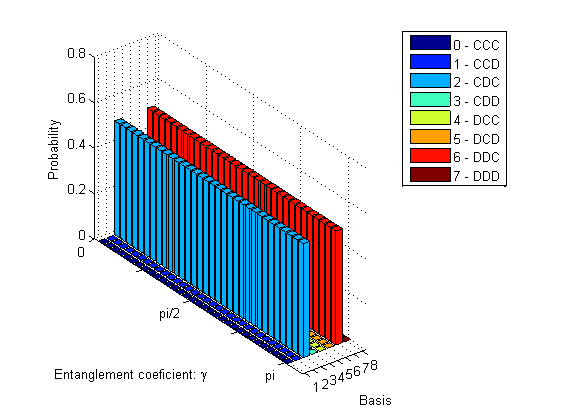
\includegraphics[scale=0.46]{3Rejected99/DCD_DD1.PNG}} \\
\end{tabular}
\caption{b) Expected utility for $3$ players, where the players will use the $(Defect, Cooperate, Defect)$ operators in the first round of the game; in the second round player 2 and player 3 will play $(DD)$. }
\label{tab:3playerDCD_DD99}
\end{center}
 \end{table}

\clearpage
\subsubsection{Initial proposal rejected; $(Defect, Defect, Cooperate)$}

\begin{table}[h]
\begin{center}
\begin{tabular}{cc}
  a)\putindeepbox[7pt]{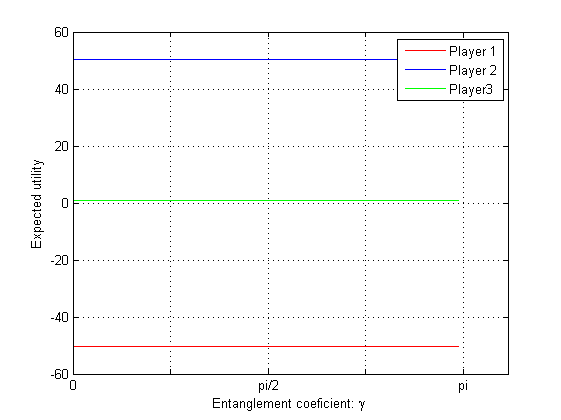
\includegraphics[scale=0.46]{3Rejected99/DDC_CC.PNG}}
    & a1)\putindeepbox[7pt]{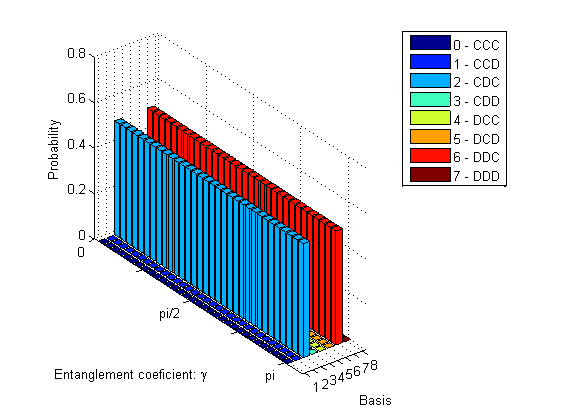
\includegraphics[scale=0.46]{3Rejected99/DDC_CC1.PNG}} \\
\end{tabular}
\caption{a) Expected utility for $3$ players, where the players will use the $(Defect, Defect, Cooperate)$ operators in the first round of the game; in the second round player 2 and player 3 will play $(CC)$. }
\label{tab:3playerDDC_CC99}
\end{center}
 \end{table}

\begin{table}[h]
\begin{center}
\begin{tabular}{cc}
  b)\putindeepbox[7pt]{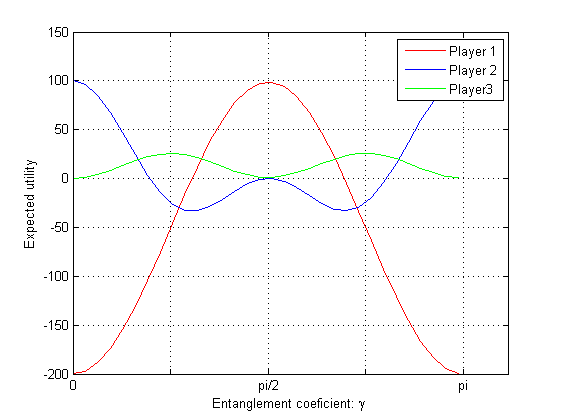
\includegraphics[scale=0.46]{3Rejected99/DDC_CD.PNG}}
    & b1)\putindeepbox[7pt]{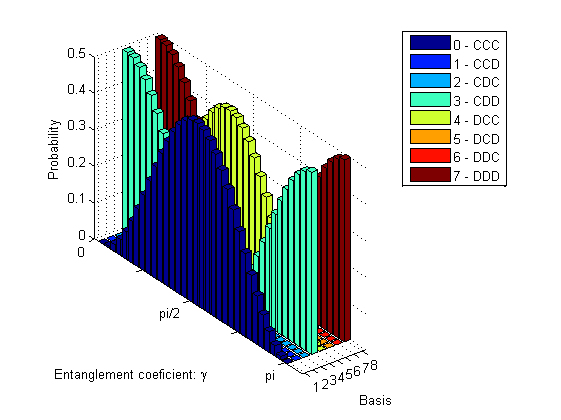
\includegraphics[scale=0.46]{3Rejected99/DDC_CD1.PNG}} \\
\end{tabular}
\caption{b) Expected utility for $3$ players, where the players will use the $(Defect, Defect, Cooperate)$ operators in the first round of the game; in the second round player 2 and player 3 will play $(CD)$. }
\label{tab:3playerDDC_CD99}
\end{center}
 \end{table}

\begin{table}[h]
\begin{center}
\begin{tabular}{cc}
  c)\putindeepbox[7pt]{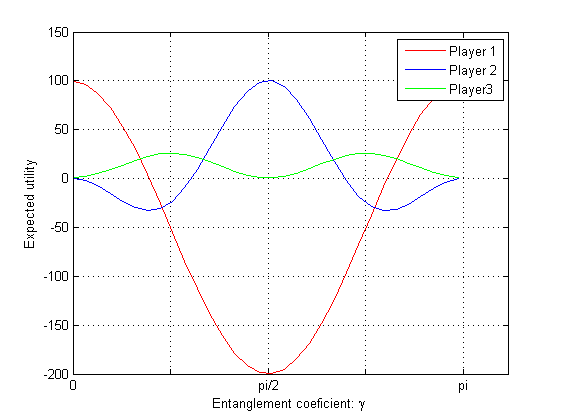
\includegraphics[scale=0.46]{3Rejected99/DDC_DC.PNG}}
    & c1)\putindeepbox[7pt]{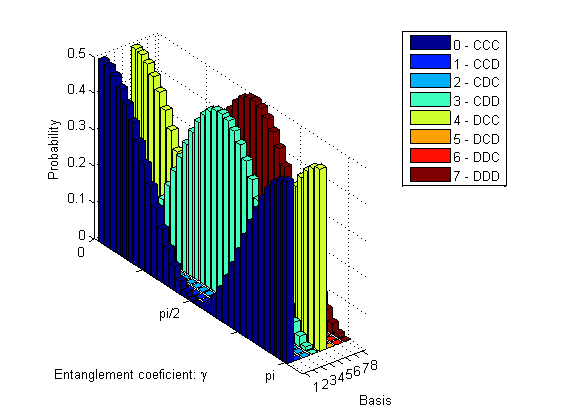
\includegraphics[scale=0.46]{3Rejected99/DDC_DC1.PNG}} \\
\end{tabular}
\caption{c) Expected utility for $3$ players, where the players will use the $(Defect, Defect, Cooperate)$ operators in the first round of the game; in the second round player 2 and player 3 will play $(DC)$. }
\label{tab:3playerDDC_DC99}
\end{center}
 \end{table}

\begin{table}[h]
\begin{center}
\begin{tabular}{cc}
  d)\putindeepbox[7pt]{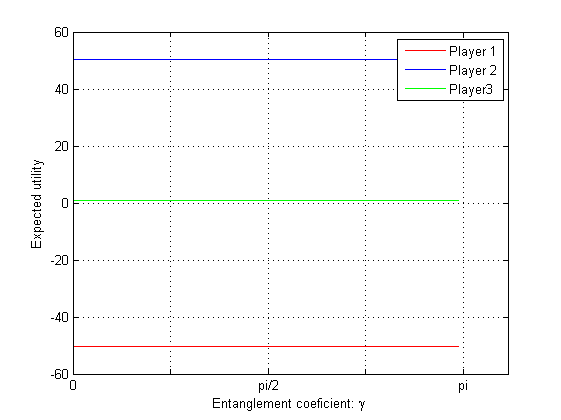
\includegraphics[scale=0.46]{3Rejected99/DDC_DD.PNG}}
    & d1)\putindeepbox[7pt]{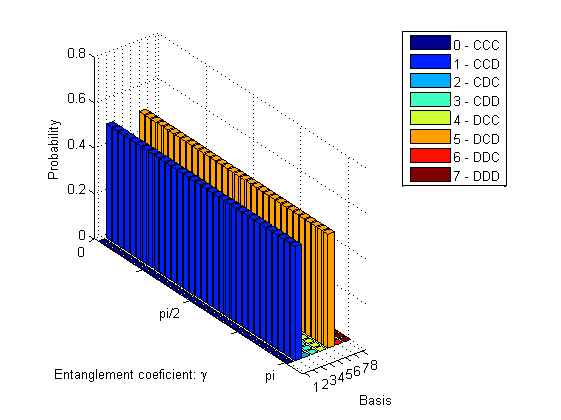
\includegraphics[scale=0.46]{3Rejected99/DDC_DD1.PNG}} \\
\end{tabular}
\caption{b) Expected utility for $3$ players, where the players will use the $(Defect, Defect, Cooperate)$ operators in the first round of the game; in the second round player 2 and player 3 will play $(DD)$. }
\label{tab:3playerDDC_DD99}
\end{center}
 \end{table}

\clearpage
\subsubsection{Initial proposal rejected; $(Defect, Defect, Defect)$}

\begin{table}[h]
\begin{center}
\begin{tabular}{cc}
  a)\putindeepbox[7pt]{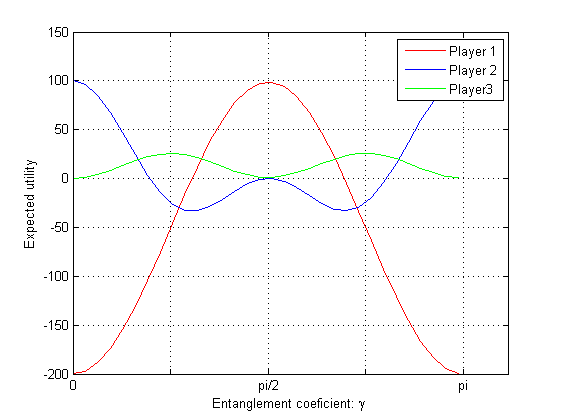
\includegraphics[scale=0.46]{3Rejected99/DDD_CC.PNG}}
    & a1)\putindeepbox[7pt]{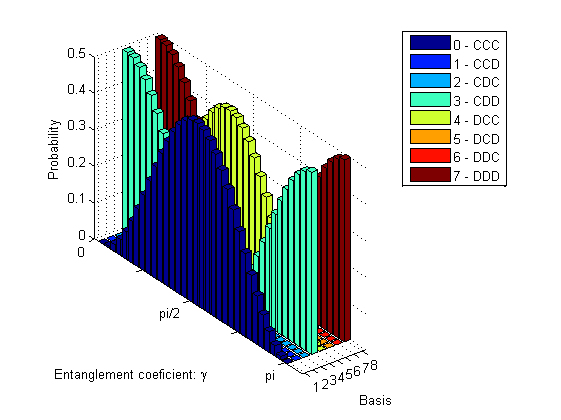
\includegraphics[scale=0.46]{3Rejected99/DDD_CC1.PNG}} \\
\end{tabular}
\caption{a) Expected utility for $3$ players, where the players will use the $(Defect, Defect, Defect)$ operators in the first round of the game; in the second round player 2 and player 3 will play $(CC)$. }
\label{tab:3playerDDD_CC99}
\end{center}
 \end{table}

\begin{table}[h]
\begin{center}
\begin{tabular}{cc}
  b)\putindeepbox[7pt]{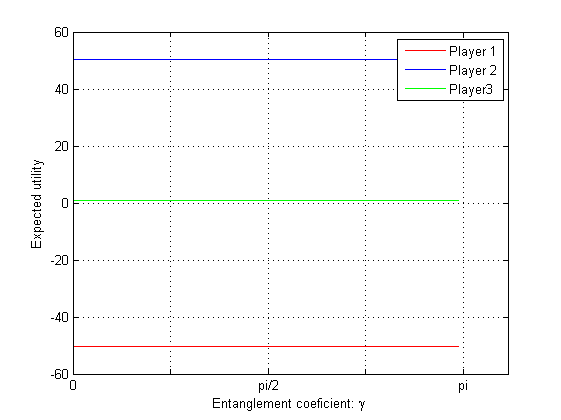
\includegraphics[scale=0.46]{3Rejected99/DDD_CD.PNG}}
    & b1)\putindeepbox[7pt]{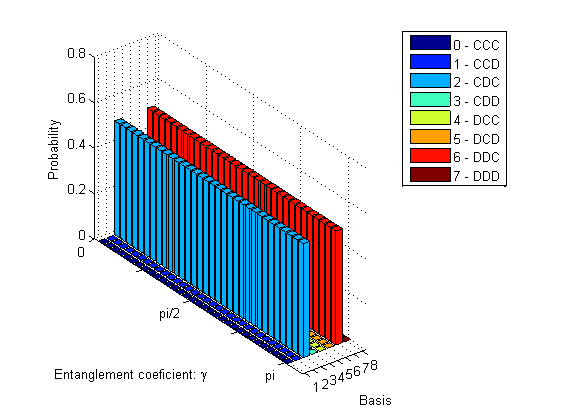
\includegraphics[scale=0.46]{3Rejected99/DDD_CD1.PNG}} \\
\end{tabular}
\caption{b) Expected utility for $3$ players, where the players will use the $(Defect, Defect, Defect)$ operators in the first round of the game; in the second round player 2 and player 3 will play $(CD)$. }
\label{tab:3playerDDD_CD99}
\end{center}
 \end{table}

\begin{table}[ht]
\begin{center}
\begin{tabular}{cc}
  c)\putindeepbox[7pt]{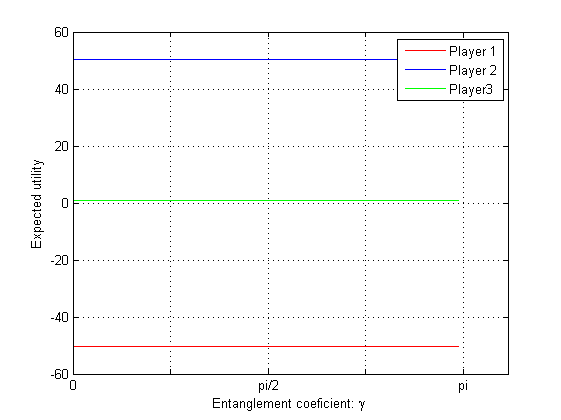
\includegraphics[scale=0.46]{3Rejected99/DDD_DC.PNG}}
    & c1)\putindeepbox[7pt]{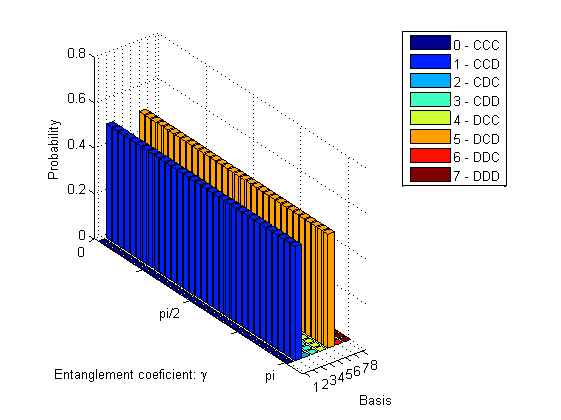
\includegraphics[scale=0.46]{3Rejected99/DDD_DC1.PNG}} \\
\end{tabular}
\caption{c) Expected utility for $3$ players, where the players will use the $(Defect, Defect, Defect)$ operators in the first round of the game; in the second round player 2 and player 3 will play $(DC)$. }
\label{tab:3playerDDD_DC99}
\end{center}
 \end{table}

\begin{table}[h]
\begin{center}
\begin{tabular}{cc}
  d)\putindeepbox[7pt]{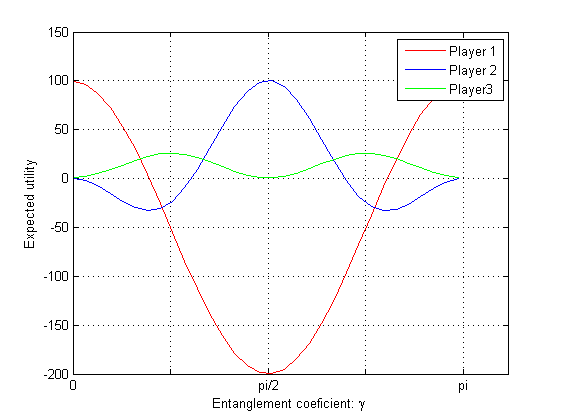
\includegraphics[scale=0.46]{3Rejected99/DDD_DD.PNG}}
    & d1)\putindeepbox[7pt]{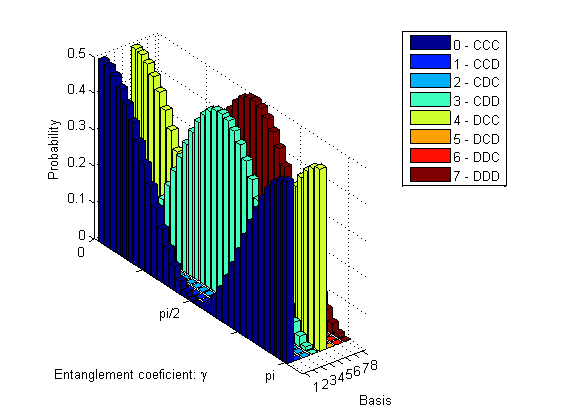
\includegraphics[scale=0.46]{3Rejected99/DDD_DD1.PNG}} \\
\end{tabular}
\caption{b) Expected utility for $3$ players, where the players will use the $(Defect, Defect, Defect)$ operators in the first round of the game; in the second round player 2 and player 3 will play $(DD)$. }
\label{tab:3playerDDD_DD99}
\end{center}
 \end{table}

%\end{itemize}

